\documentclass[12pt]{article}
\usepackage{amssymb}
\usepackage[english]{babel}
\usepackage{fullpage}
\usepackage{graphicx,multirow}
\usepackage{caption}
\usepackage[margin=1.52in]{geometry}
\captionsetup{font=bf,belowskip=11pt}
\usepackage{hyperref}
\usepackage{amsmath}
\usepackage{enumitem}
\usepackage{subfig}
\usepackage{placeins}
\usepackage{tabularray}
\usepackage{float}


\begin{document}
\begin{titlepage} 
	\newcommand{\HRule}{\rule{\linewidth}{0.5mm}}
	\center
	\textsc{\LARGE Polytechnique Montréal}\\[1.5cm]
	\textsc{\Large LOG8415 : Lab 2}\\[0.5cm]
	\textsc{\large Advanced Concepts in Cloud Computing}\\[0.5cm]
	\HRule\\[0.4cm]
	{\huge\bfseries MapReduce with Hadoop on AWS (or Azure)}\\[0.4cm]
	\HRule\\[1.5cm]
	{\large\textit{Authors}}\\
	Anis \textsc{Zouatene} (1963304)\\
	Aleksandar \textsc{Stijelja} (1959772)\\
	Amin \textsc{Ghadesi} (2121658)\\
    Reza \textsc{Rouhghalandari} (2153395)\\
	\vfill\vfill\vfill {\large\today} \vfill\vfill
	
\includegraphics{poly-logo.png}\\[1cm]
	\vfill
\end{titlepage}


\section{Abstract}
	\paragraph{} The programming model known as "MapReduce" facilitates concurrent processing by splitting 
	petabytes of data into smaller chunks, and processing them in parallel on Hadoop commodity servers. 
	In the end, it aggregates all the data from multiple servers to return a consolidated output back to 
	the application.
		
	\paragraph{} However we have different ways to manage Big Data sets, such as Apache Hadoop or Apache 
	Spark. In this paper, we will explore both softwares and compare their differences and evaluate their 
	performances by conducting a few experiments.

	\paragraph{Keywords:}Big Data, Azure, MapReduce, Spark, Hadoop, Big Data.
	\pagebreak

\section{Introduction}
	\paragraph{} As such, in this lab we compared the performance of the algorithm on Linux, Hadoop and Spark with 
	different experiments. We began by comparing  their performances in a simple WordCount program and noted their 
	differences. The WordCount program counts the occurrence of every single word in the specified document. 
	To do this, we chose to use Azure instead of AWS. We then created a VM in it, then we used Hadoop and MapReduce 
	to solve a social networking problem and process bigger data sets.
	\bigskip

	\paragraph{} In this lab, we will be presenting the experiments done with WordCount program, the performance 
	comparison of Hadoop vs Linux, the performance comparison of Hadoop vs Spark on Azure and the people you might
	know algorithm problem. 

	\bigskip

	\pagebreak

\section{Experiments with WordCount program}
	\paragraph{} Before getting into the performance experiments between Hadoop, Spark and Linux, 
	we began by experimenting with the WordCount program java example given with both Hadoop and Spark. 
	After installing the required Java packages and setting up all environment variables required, we 
	proceeded to run the WordCount example on a copy of pg4300.txt. We made use of the TIME command to
	be able to extract the time performance of the run. It would provide us with the "real", "user" and
	"sys" duration of the command executed.

	\begin{figure}[H]
	\centering
	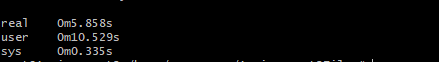
\includegraphics[width=140mm, scale=0.5]{images/hadoop-time.png}
	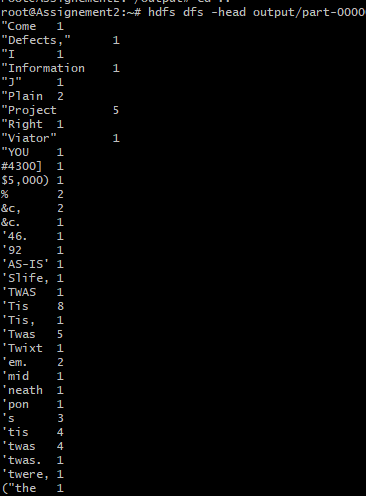
\includegraphics[width=80mm, scale=0.75]{images/output-pg4300.png}
	\caption*{\textbf{Figure 1}: Result of Hadoop WordCount.java on pg3000.txt}
	\end{figure}

\section{Performance comparison of Hadoop vs Linux}
    \paragraph{} Now that we experimented using Hadoop with the wordcount example talked previously, 
	we can now start running Hadoop WordCount on all the datasets provided and compare with Linux. 
	We had to do 3 tests on each to get an average for both. Here are the results.

	\begin{figure}[H]
	\centering
	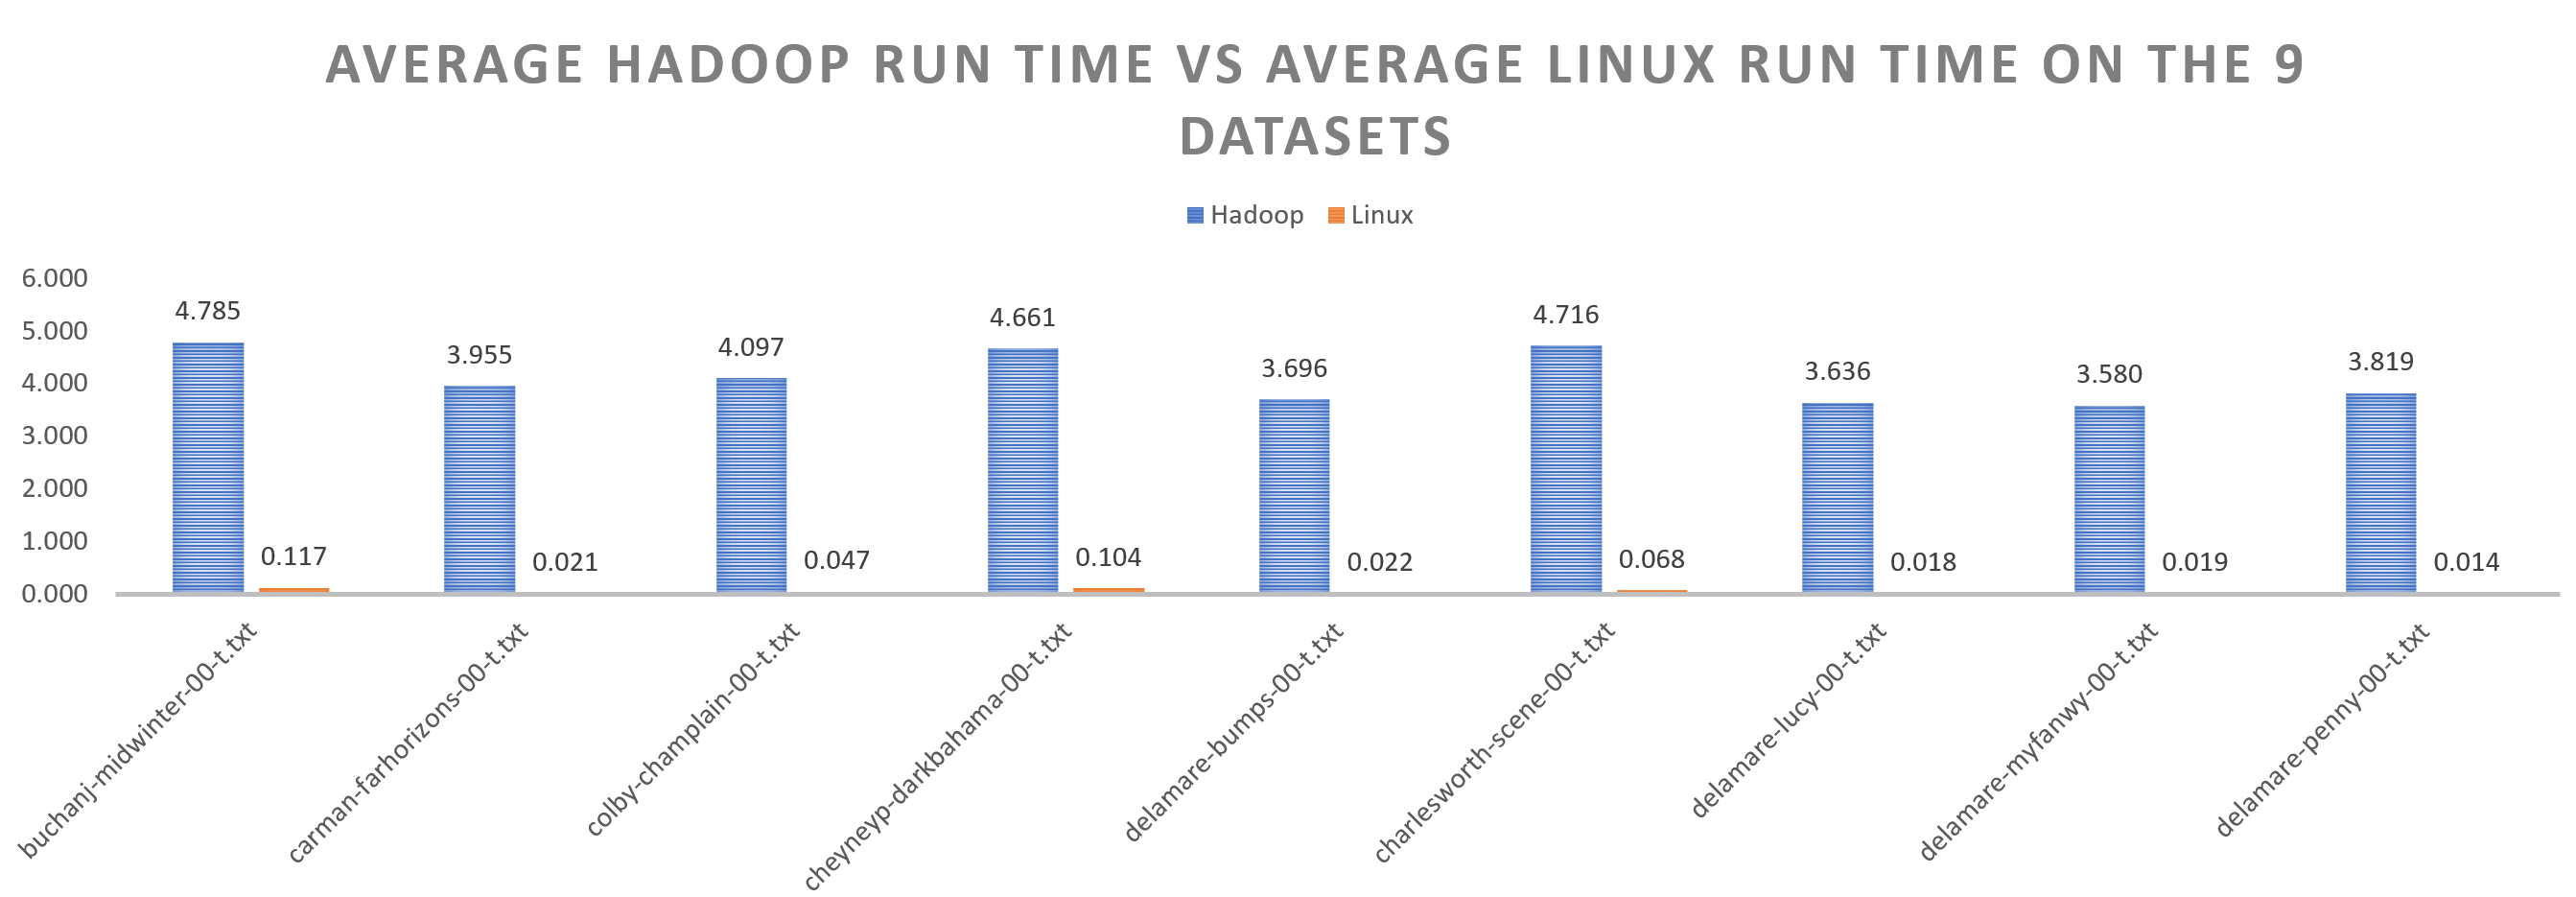
\includegraphics[width=160mm, height=70mm, scale=1.0]{images/Hadoop_vs_Linux_graph.PNG}
	\caption*{\textbf{Figure 1}: Result of Hadoop vs Linux runtime}
	\end{figure}
		
	\begin{figure}[H]
	\centering
	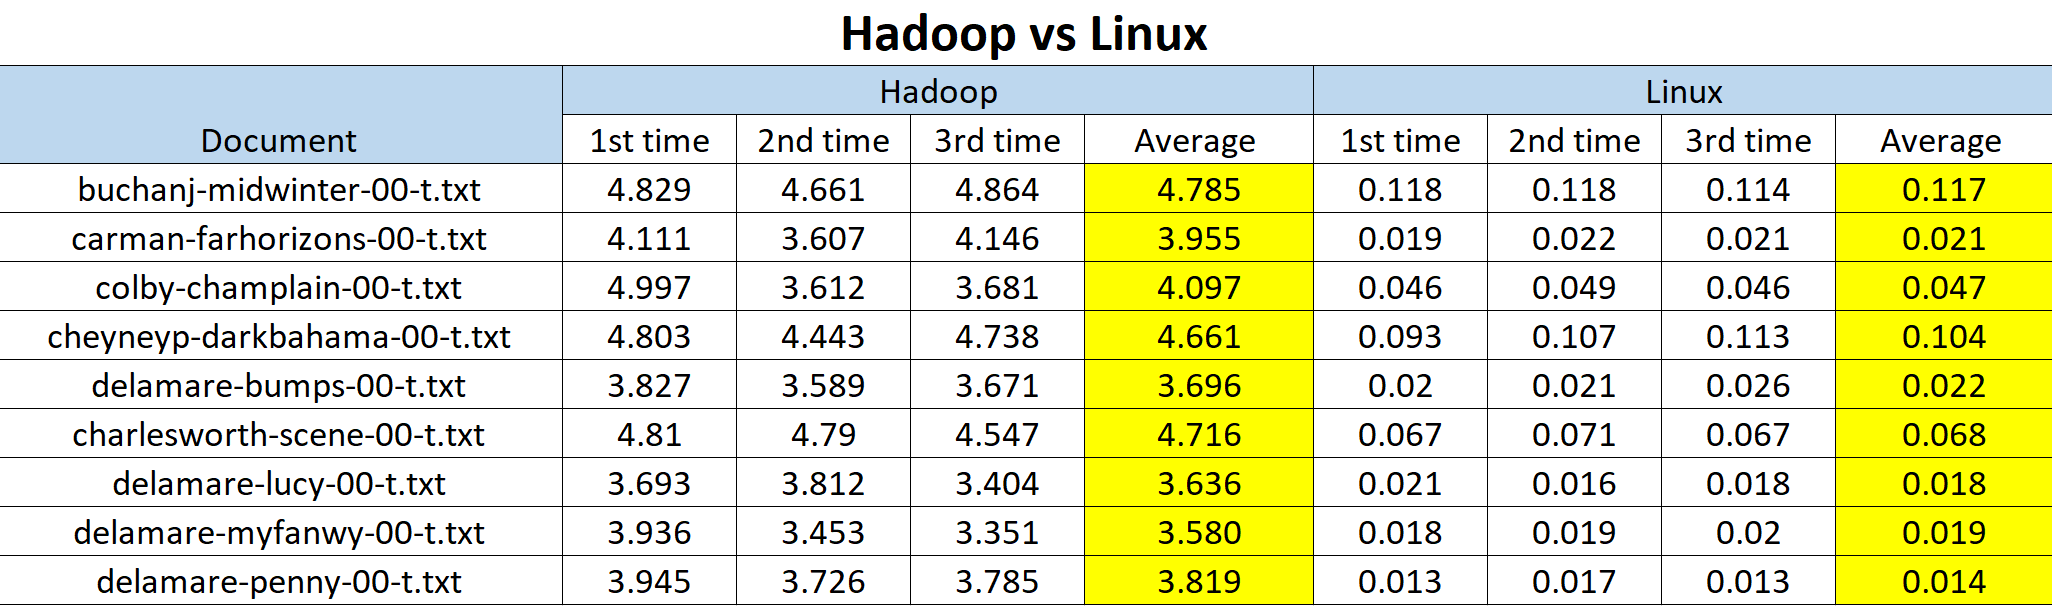
\includegraphics[width=160mm, height=60mm, scale=1.0]{images/Hadoop_vs_Linux_table.PNG}
	\caption*{\textbf{Figure 1}: Average run time of Hadoop vs Linux on each dataset}
	\end{figure}

	\subsection{Results}
        \paragraph{} By looking at the results above, we can see that Linux outperformed Hadoop 
		by a LOT. One of the reasons for this kind of result is that Hadoop is meant to process 
		very large sets of data, as such given this set of small data, Linux was able to outperform 
		Hadoop. This doesn't mean that Hadoop is inferior, because if we are dealing with large quantities 
		of data, then we expect Hadoop to outperform easily Linux.
        \bigskip

\section{Performance comparison of Hadoop vs Spark on Azure}
	\paragraph{} Using the same Azur VM used previously, we used the same method that was used for Hadoop 
	vs Linux. As such to properly evaluate both Hadoop and Spark, we ran the WordCount with the command 
	TIME 3 times on each dataset for both. The difference was that, for Spark we used the code in Python. 
	The file is named SparkWordCount.py.
	\paragraph{} The command used for Hadoop began with "time hadoop ...", whereas that with Spark began 
	with "time spark-submit ...". This information is presented in more details in our readme.md.

	\begin{figure}[H]
	\centering
	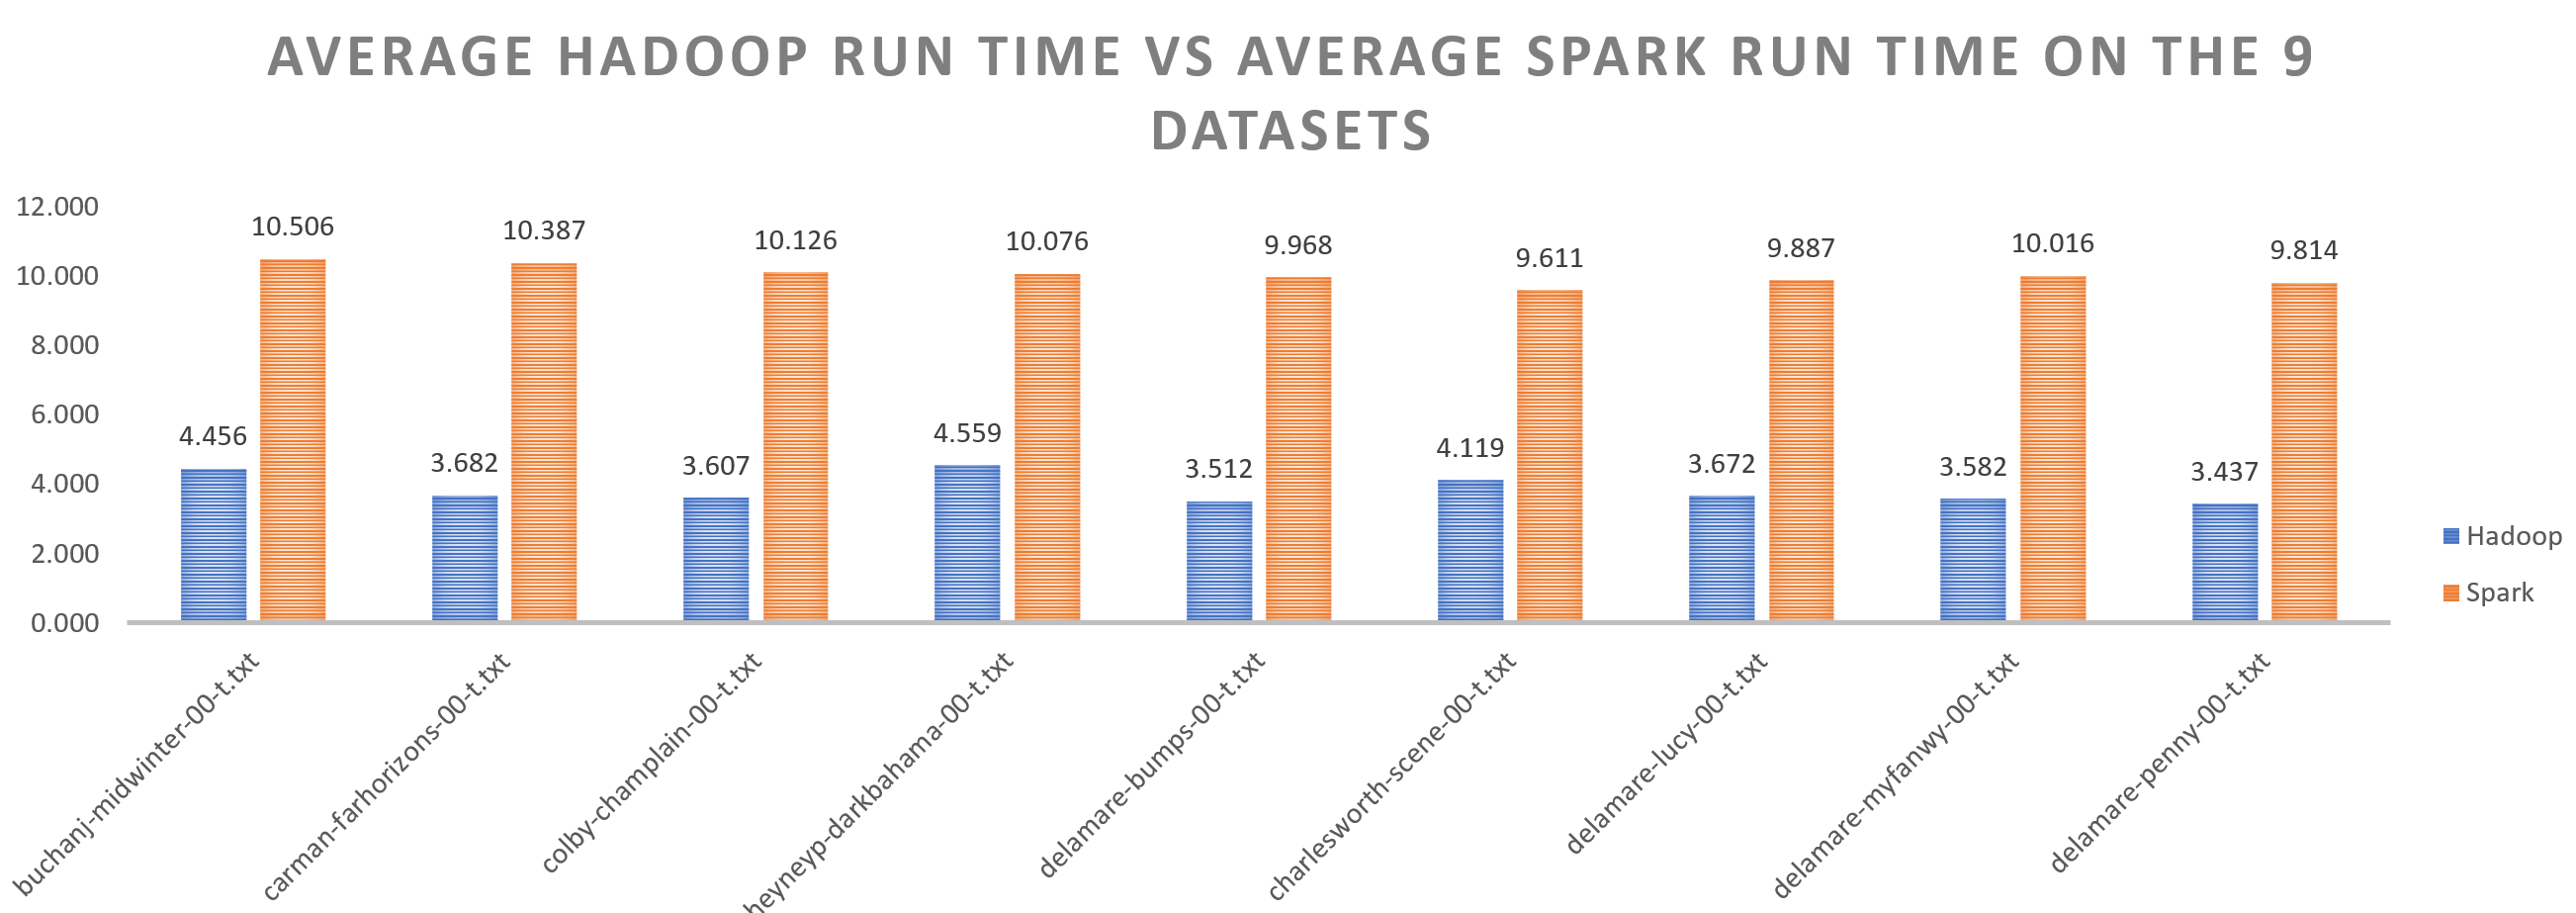
\includegraphics[width=160mm, height=70mm, scale=1.0]{images/Hadoop_vs_Spark_graph.PNG}
	\caption*{\textbf{Figure 4}: Result of Hadoop vs Spark on each dataset}
	\end{figure}
	
	\begin{figure}[H]
	\centering
	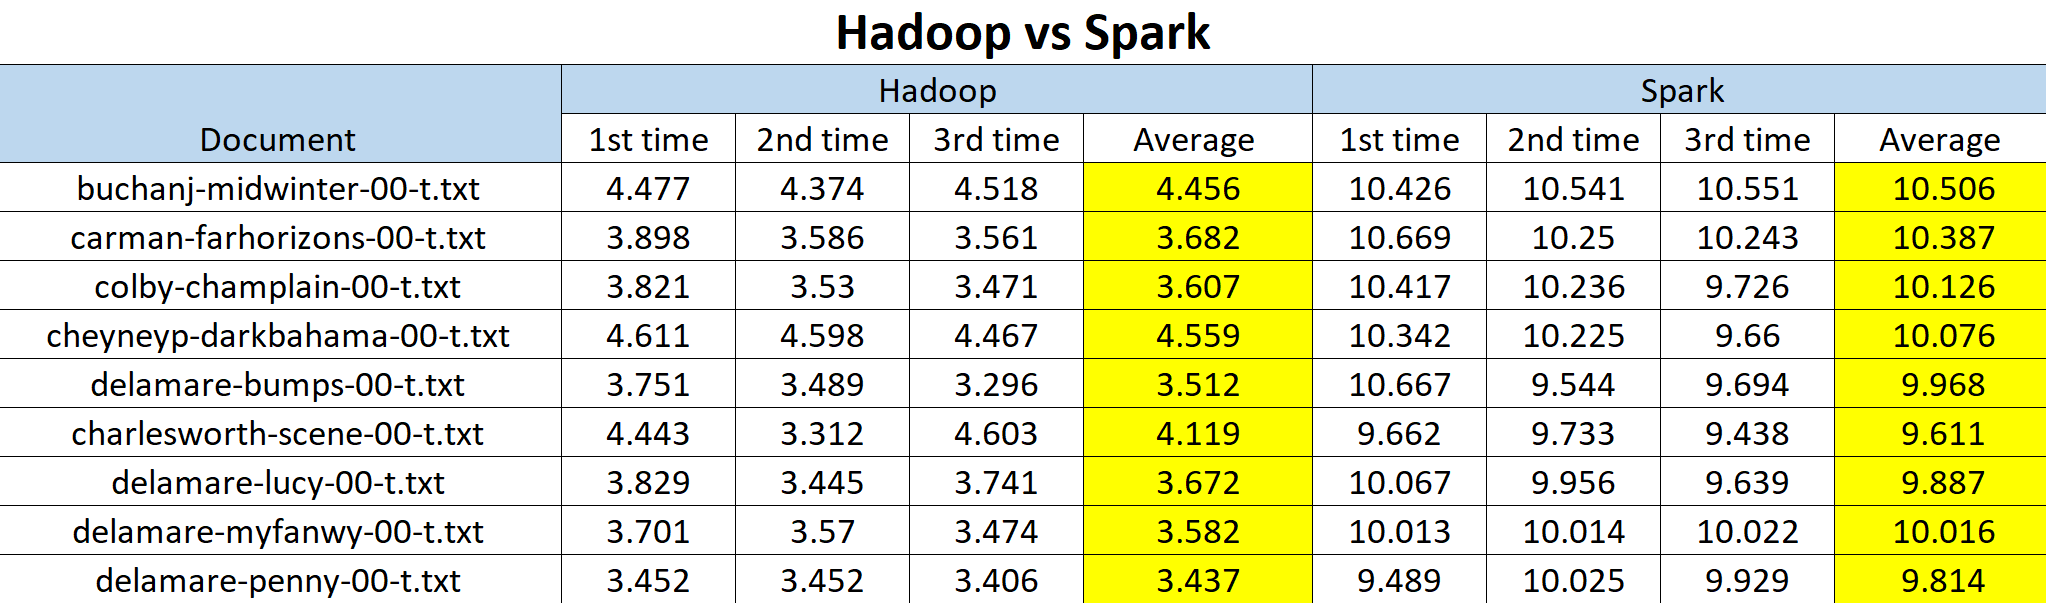
\includegraphics[width=160mm, height=70mm, scale=1.0]{images/Hadoop_vs_Spark_table.PNG}
	\caption*{\textbf{Figure 5}: Average run time of Hadoop vs Spark on each dataset}
	\end{figure}
	
	\subsection{Results}
		\paragraph{} 
		\bigskip
		
\end{document}